\chapter{Fitting and Interpreting GLMs \label{chapter:fitglm}}

Generalized linear models (Chapter~\ref{chapter:glms}) are just one way to approach supervised learning. However, they are by far the most common approach in the clinical research literature. Linear and logistic regression are established, standard methods for clinical data analysis in contexts where you want to relate the effects of one or more predictors to an outcome that is a number or a class (e.g. yes/no). Because of this, it is important to know how to interpret these models -- e.g., what the coefficients, standard errors, and model diagnostics mean -- and how to fit them using software. 

%%%%%%%%%%%%%%%%%%%%%%%%%%%%%%%%%%%%%%%%%%%%%%%%%%%%%%%%%%%%%%%%%%%%%%%%%%%%%%%

\section{Examples from Chapters~\ref{chapter:classification} and \ref{chapter:regression} \label{sect:clregexamples}}

In Chapter~\ref{chapter:classification}, we saw an example where information about two predictors -- a disease severity score ($x_1$) and a social determinants score ($x_2$) -- was used to predict a binary outcome: whether a patient would be readmitted to the ER within 30 days of discharge. In Chapter~\ref{chapter:regression}, we used the same two predictors to predict the numeric level of a disease recurrence biomarker. Here are pictures of the logistic regression model from Chapter~\ref{chapter:classification} and the linear regression model from Chapter~\ref{chapter:regression} with their fitted model summary output. Note: These pictures include axis labels, whereas those from Chapters~\ref{chapter:classification} and \ref{chapter:regression} did not. 

\begin{center}
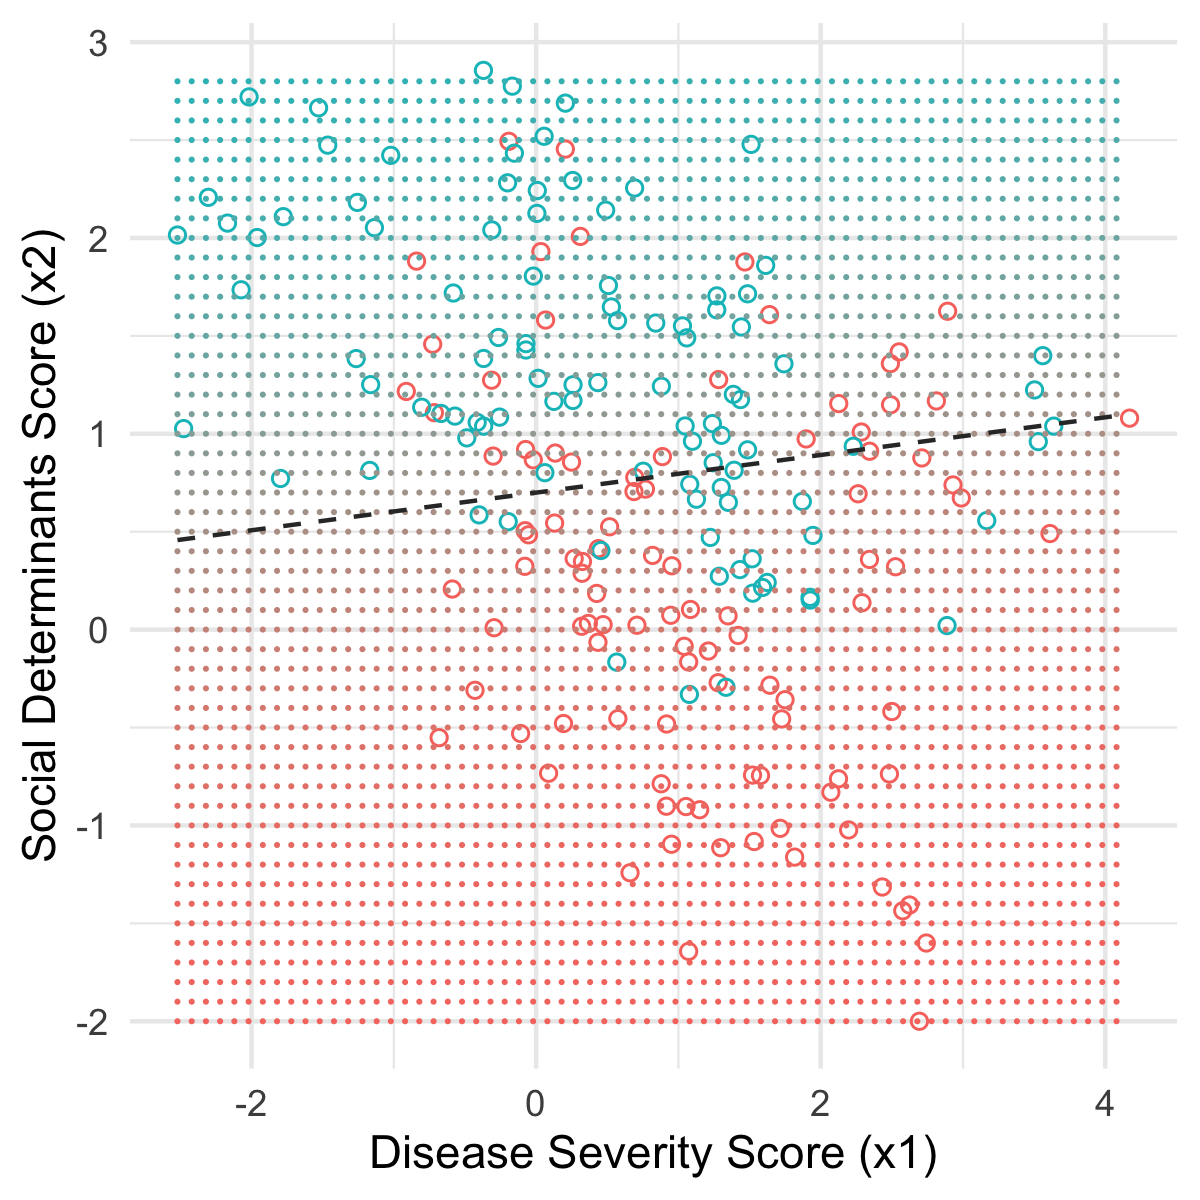
\includegraphics[width=0.35\textwidth]{img/esl-logistic-prob-axes.png}
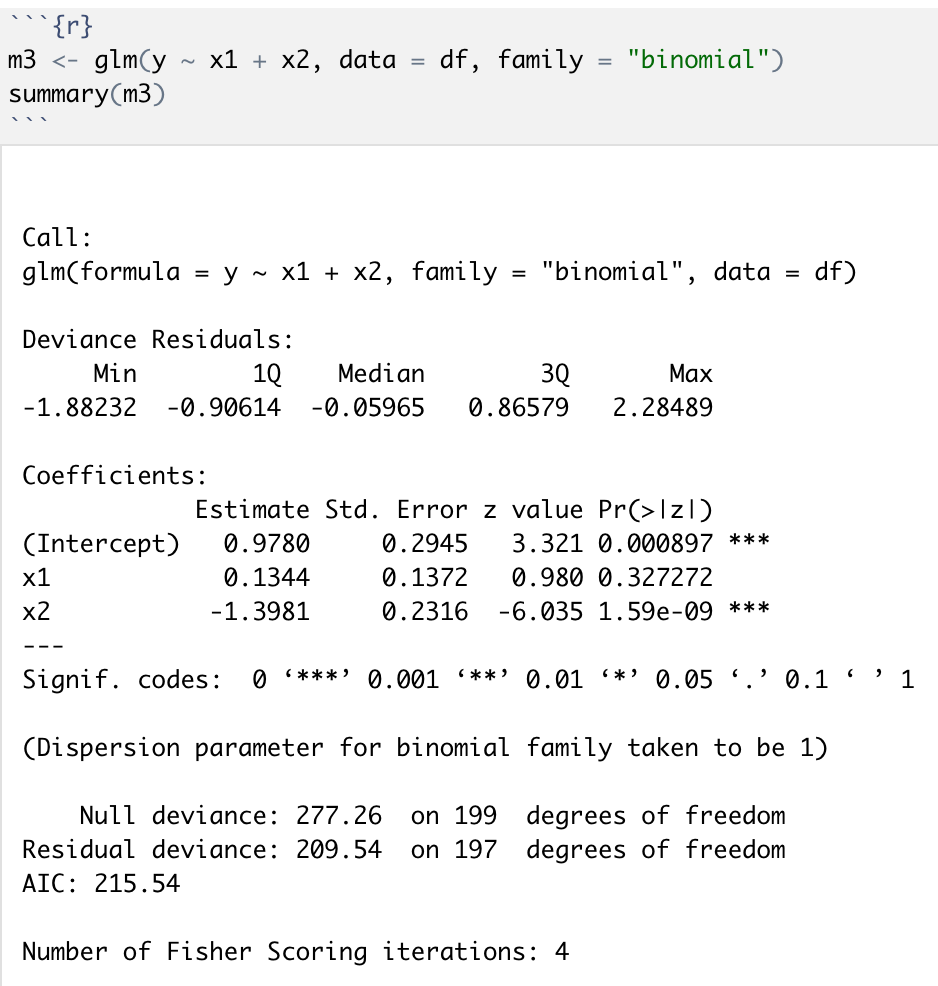
\includegraphics[width=0.64\textwidth]{img/glm-binomial-example.png}\\[8mm]
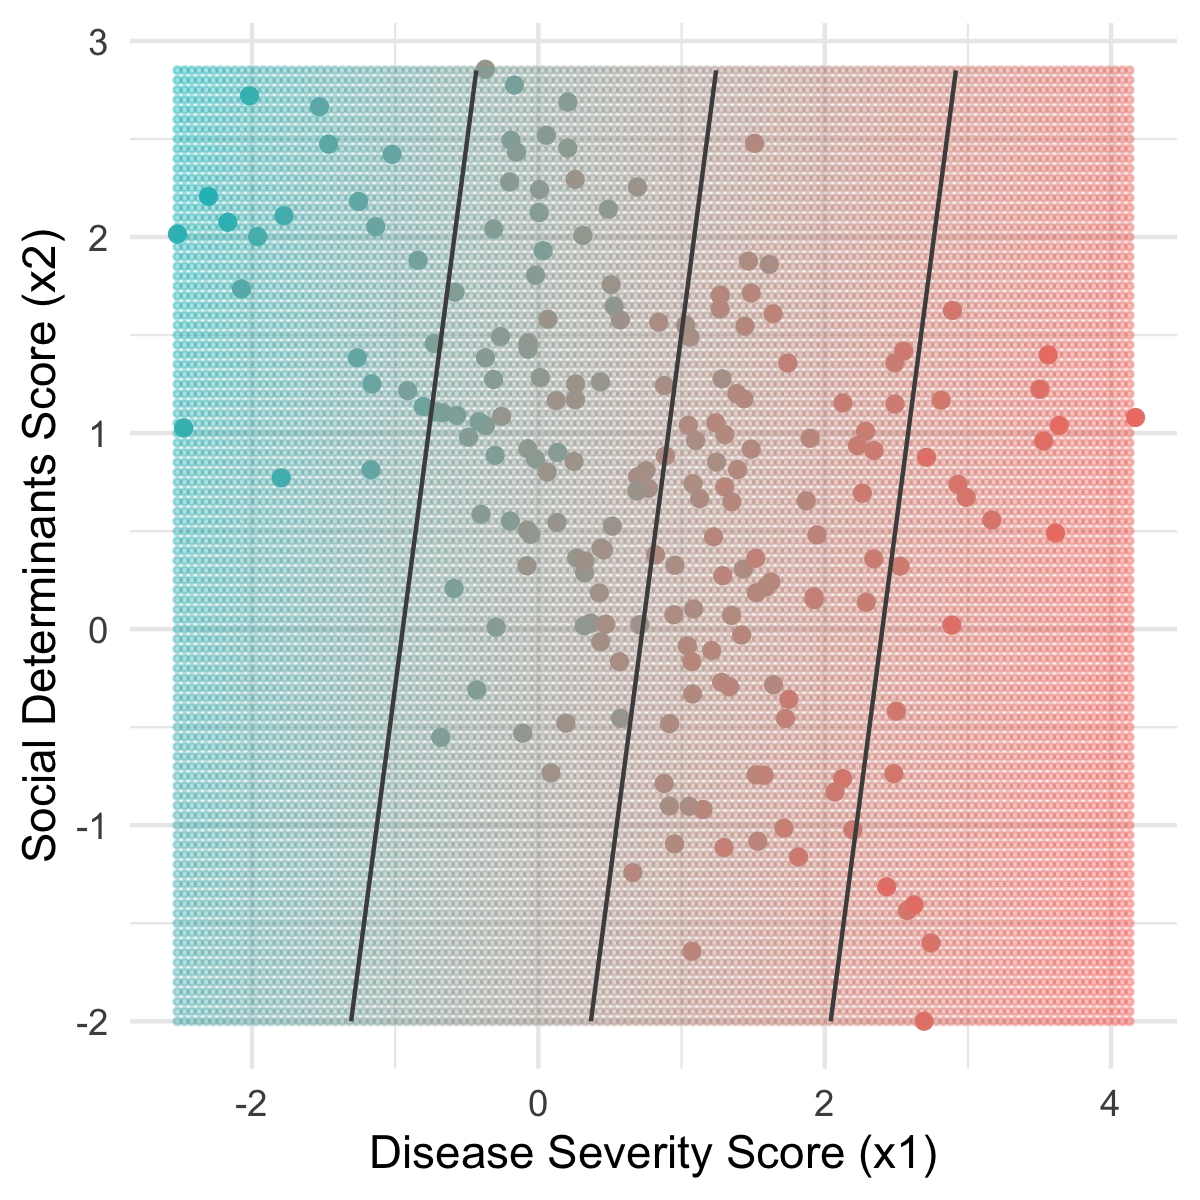
\includegraphics[width=0.35\textwidth]{img/esl-reg-linear-wlabels.png}
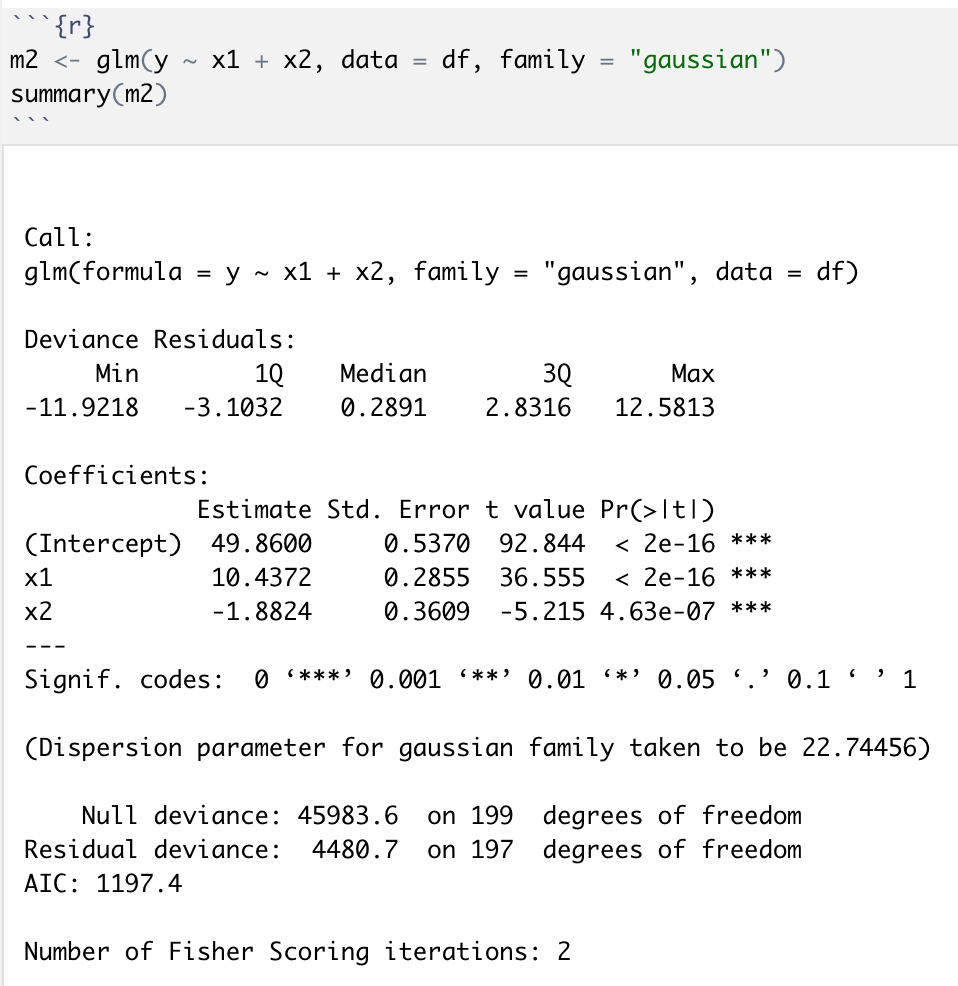
\includegraphics[width=0.64\textwidth]{img/glm-gaussian-example.png}
\end{center}

\begin{question}{}
Interpret the meaning of the coefficients of $x_1$ and $x_2$ in the linear regression model.
\end{question}

\begin{question}{}
Interpret the meaning of the intercept in the linear regression model.
\end{question}

\begin{question}{}
Interpret the meaning of the coefficients of $x_1$ and $x_2$ in the logistic regression model.
\end{question}

\begin{question}{}
Interpret the meaning of the intercept in the logistic regression model.
\end{question}

%%%%%%%%%%%%%%%%%%%%%%%%%%%%%%%%%%%%%%%%%%%%%%%%%%%%%%%%%%%%%%%%%%%%%%%%%%%%%%%

\section{Standard Errors and Hypothesis Tests}

The magnitudes of the coefficients in these models matter only in relation to:
\begin{enumerate}
\item The scale on which the predictors are measured. 
\item The amount of uncertainty the model has about their values.
\end{enumerate}
For example, if a predictor varies only across a tiny range of values, its model coefficient may be large, since it quantifies the change in the link-function-transformed outcome when the predictor changes by 1.0. However, that doesn't mean that the predictor itself is important to the outcome\footnote{This is one reason many advocate \textbf{scaling} and \textbf{centering} predictors before fitting a model. Centering means subtracting the mean value of a predictor from all of its individual measurements so that the mean of each centered predictor is zero. Scaling means dividing the values of each predictor by their standard deviation, so that the standard deviation of each predictor is 1.0. This enables the relative magnitudes of the model coefficients to be compared directly.}.

Similarly, the model may be highly uncertain about a coefficient's value, owing to factors like a small dataset (small $n$) or collinearity among the predictors. Mathematically, high uncertainty means that the value of the likelihood doesn't change very rapidly as you move away from the maximum likelihood estimate of a coefficient. For example, here is how the log-likelihood for the logistic regression example above changes when we vary $\beta_1$ (the coefficient of $x_1$), keeping $\beta_0$ (the intercept) and $\beta_2$ (the coefficient of $x_2$) fixed at their MLEs: 
\begin{center}
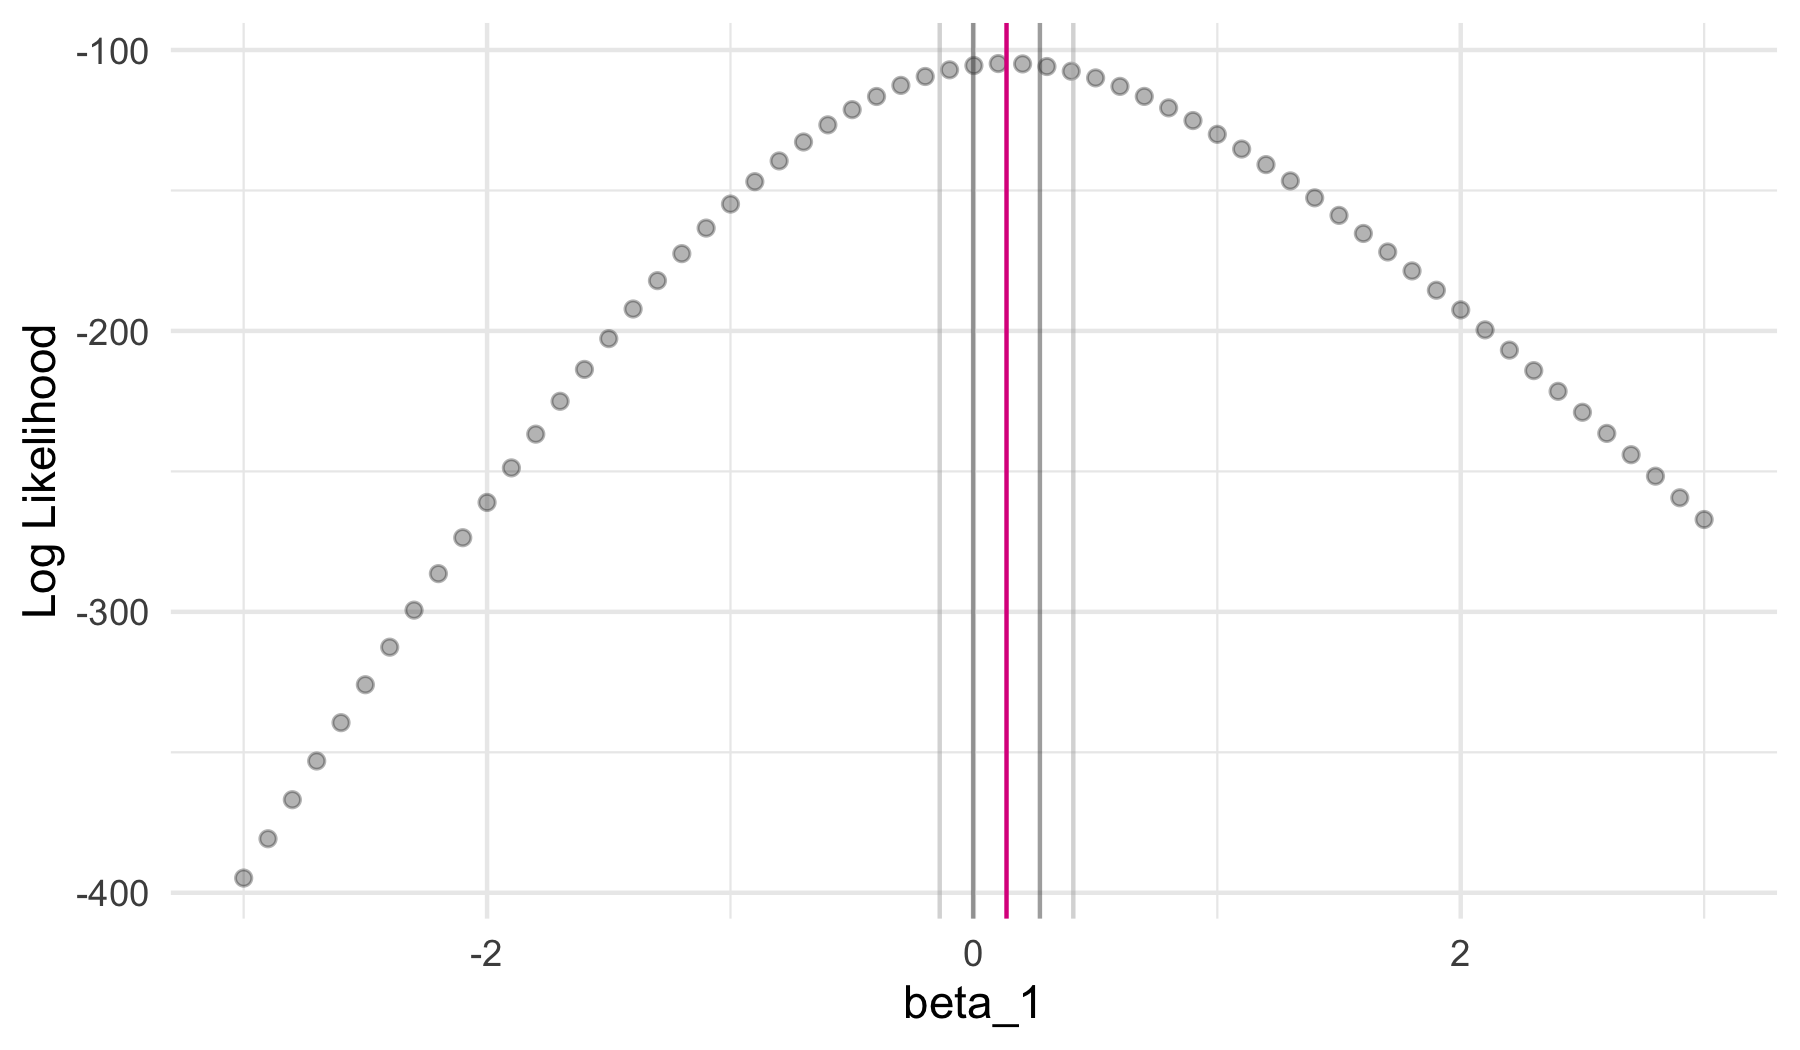
\includegraphics[width=0.7\textwidth]{img/esl-logistic-beta1.png}
\end{center}
The gray vertical lines are related to the \textbf{standard error} of the model coefficient, which is in turn related to the ``flatness'' of the likelihood surface around the MLE. The gray lines are situated at 1 and 2 standard errors away from the MLE in either direction. You can see that in the case of $\beta_1$, the gray lines overlap zero. The value zero (no effect) is a plausible estimate of the impact of $x_1$ on the outcome. 

Contrast this with how the log-likelihood varies around the MLE for $\beta_2$:
\begin{center}
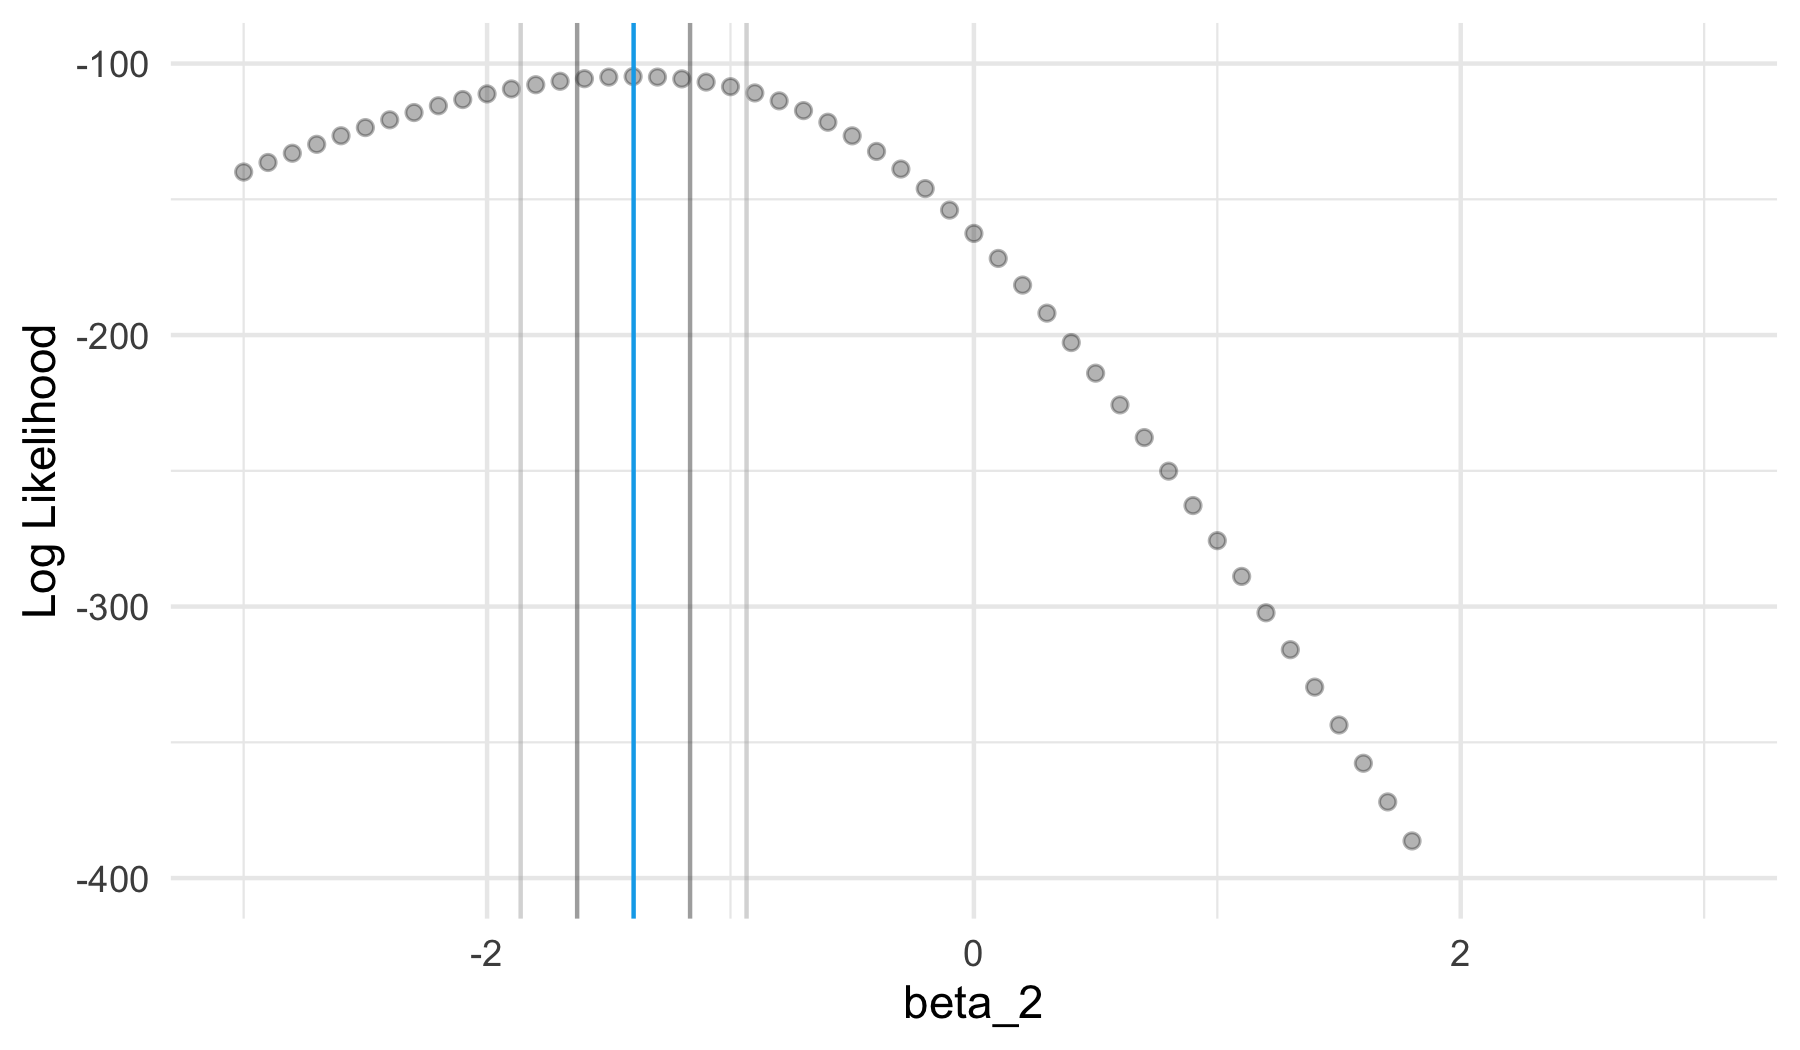
\includegraphics[width=0.7\textwidth]{img/esl-logistic-beta2.png}
\end{center}
Here the standard error is larger, but the magnitude of the coefficient is also larger, so the range of the gray lines does not overlap zero. These findings are reflected in the relative values of the \textbf{Z-statistic} (\texttt{z value}) and \textbf{P-value} (\verb|Pr(>|z|)|) in the model output for the two coefficients. Whether a coefficient's value is likely to be nonzero is typically evaluated using a formalism called a \textbf{hypothesis test}. We will discuss hypothesis tests in much greater detail in Chapter~\ref{chapter:hypothesistesting}.  

%%%%%%%%%%%%%%%%%%%%%%%%%%%%%%%%%%%%%%%%%%%%%%%%%%%%%%%%%%%%%%%%%%%%%%%%%%%%%%%

\section{Case Study: Linear Regression}

The following data come from an early study that examined the possible link between air pollution and mortality. The authors examined 60 cities throughout the United States and recorded the following data:
\begin{center}
\texttt{ \small \begin{tabular}{ll}
\toprule
MORT & Total age-adjusted mortality from all causes, \\
& in deaths per 100,000 population \\
PRECIP & Mean annual precipitation (in inches) \\
EDUC & Median number of school years completed \\
& for persons of age 25 years or older \\
NONWHITE & Percentage of the 1960 population that is nonwhite \\
NOX & Relative pollution potential of oxides of nitrogen \\
SO2 & Relative pollution potential of sulfur dioxide \\
\bottomrule
\end{tabular}
}
\end{center}
Note: ``Relative pollution potential'' refers to the product of the tons emitted per day per square kilometer and a factor correcting the SMSA dimensions and exposure.

We want to predict the value of \texttt{MORT} ($y$) using the predictors \texttt{PRECIP, EDUC, NONWHITE, NOX,} and \verb|SO2| ($x_1, x_2, x_3, x_4$ and $x_5$). Here is the GLM output for this model in R:
{\small
\begin{verbatim}
Call:
glm(formula = MORT ~ PRECIP + EDUC + NONWHITE + NOX + SO2, 
    family = "gaussian", data = d)

Deviance Residuals: 
   Min      1Q  Median      3Q     Max  
-91.38  -18.97   -3.56   16.00   91.83  

Coefficients:
             Estimate Std. Error t value Pr(>|t|)    
(Intercept) 995.63646   91.64099  10.865 3.35e-15 ***
PRECIP        1.40734    0.68914   2.042 0.046032 *  
EDUC        -14.80139    7.02747  -2.106 0.039849 *  
NONWHITE      3.19909    0.62231   5.141 3.89e-06 ***
NOX          -0.10797    0.13502  -0.800 0.427426    
SO2           0.35518    0.09096   3.905 0.000264 ***
---
Signif. codes:  0 '***' 0.001 '**' 0.01 '*' 0.05 '.' 0.1 ' ' 1

(Dispersion parameter for gaussian family taken to be 1375.723)

    Null deviance: 228275  on 59  degrees of freedom
Residual deviance:  74289  on 54  degrees of freedom
AIC: 611.56

Number of Fisher Scoring iterations: 2
\end{verbatim}
}

Side note: Most models can be fit multiple ways. Linear regression models are normally fit using \textbf{ordinary least squares} and the \verb|lm| package, as opposed to maximum likelihood and the \verb|glm| package. The coefficients and most of the output are exactly the same:

{\small
\begin{verbatim}
Call:
lm(formula = MORT ~ PRECIP + EDUC + NONWHITE + NOX + SO2, 
   data = d)

Residuals:
   Min     1Q Median     3Q    Max 
-91.38 -18.97  -3.56  16.00  91.83 

Coefficients:
             Estimate Std. Error t value Pr(>|t|)    
(Intercept) 995.63646   91.64099  10.865 3.35e-15 ***
PRECIP        1.40734    0.68914   2.042 0.046032 *  
EDUC        -14.80139    7.02747  -2.106 0.039849 *  
NONWHITE      3.19909    0.62231   5.141 3.89e-06 ***
NOX          -0.10797    0.13502  -0.800 0.427426    
SO2           0.35518    0.09096   3.905 0.000264 ***
---
Signif. codes:  0 '***' 0.001 '**' 0.01 '*' 0.05 '.' 0.1 ' ' 1

Residual standard error: 37.09 on 54 degrees of freedom
Multiple R-squared:  0.6746,  Adjusted R-squared:  0.6444 
F-statistic: 22.39 on 5 and 54 DF,  p-value: 4.407e-12
\end{verbatim}
}

\begin{question}{}
Interpret the values of each of these coefficients. Based on the coefficient values and their standard errors, which predictor(s) do you think have the greatest impact on mortality? 
\end{question}

\begin{question}{}
In this model, is the effect of one predictor (say, \verb|PRECIP|) impacted by the value(s) of any of the other predictor(s)? How does this differ from the other regression algorithms we've seen (KNN and decision trees)? What are the advantages and disadvantages of this choice? 
\end{question}

%%%%%%%%%%%%%%%%%%%%%%%%%%%%%%%%%%%%%%%%%%%%%%%%%%%%%%%%%%%%%%%%%%%%%%%%%%%%%%%

\section{Case Study: Logistic Regression}

The goal of this study was to identify risk factors associated with giving birth to a low birth weight baby (a baby weighing less than 2500 grams). Infant mortality rates and birth defect rates are very high for low birth weight babies. A woman's behavior during pregnancy (including diet, smoking habits, and receiving prenatal care) can greatly alter the chances of carrying the baby to term and, consequently, of delivering a baby of normal birth weight.

Data were collected on 189 women, 59 of which had low birth weight babies and 130 of which had normal birth weight babies.

\begin{center}
\texttt{ \small
\begin{tabular}{ll}
\toprule
LOW & Low birth weight (0 = birth weight $\geq$ 2500 g;\\
& 1 = birth weight $< 2500$ g) \\
AGE & Age of mother in years \\
LWT & Mother's weight in pounds at last menstrual period \\
RACE & Race (1 = white, 2 = black, 3 = other) \\
SMOKE & Smoking status during pregnancy (1 = yes, 0 = no) \\
PTL & History of premature labor (0 = none, 1 = one, etc.) \\
HT & History of hypertension (0 = no, 1 = yes) \\
UI & Presence of uterine irritability (0 = no, 1 = yes) \\
FTV & Number of physician visits during the first trimester \\
BWT & Birth weight in grams \\
\bottomrule
\end{tabular}
}
\end{center}
SOURCE: Hosmer and Lemeshow (2000) \emph{Applied Logistic Regression: Second Edition}. Data were collected at Baystate Medical Center, Springfield, Massachusetts during 1986. 

We would like to predict \texttt{LOW} based on all of the other covariates except \texttt{BWT}. (Why not use \texttt{BWT}?) The GLM output of this model is:

{\small
\begin{verbatim}
Call:
glm(formula = LOW ~ AGE + LWT + RACE + SMOKE + PTL + HT + UI + 
    FTV, family = "binomial", data = d)

Deviance Residuals: 
    Min       1Q   Median       3Q      Max  
-1.8946  -0.8212  -0.5316   0.9818   2.2125  

Coefficients:
             Estimate Std. Error z value Pr(>|z|)   
(Intercept)  0.480623   1.196888   0.402  0.68801   
AGE         -0.029549   0.037031  -0.798  0.42489   
LWT         -0.015424   0.006919  -2.229  0.02580 * 
RACE2        1.272260   0.527357   2.413  0.01584 * 
RACE3        0.880496   0.440778   1.998  0.04576 * 
SMOKE        0.938846   0.402147   2.335  0.01957 * 
PTL          0.543337   0.345403   1.573  0.11571   
HT           1.863303   0.697533   2.671  0.00756 **
UI           0.767648   0.459318   1.671  0.09467 . 
FTV          0.065302   0.172394   0.379  0.70484   
---
Signif. codes:  0 '***' 0.001 '**' 0.01 '*' 0.05 '.' 0.1 ' ' 1

(Dispersion parameter for binomial family taken to be 1)

    Null deviance: 234.67  on 188  degrees of freedom
Residual deviance: 201.28  on 179  degrees of freedom
AIC: 221.28

Number of Fisher Scoring iterations: 4
\end{verbatim}
}

\begin{question}{}
In this model, is the effect of one predictor (say, \verb|AGE|) impacted by the value(s) of any of the other predictor(s)? How does this differ from the other classification algorithms we've seen (KNN and decision trees)? What are the advantages and disadvantages of this choice? 
\end{question}

\begin{question}{}
Comment on how the variable \texttt{RACE} enters into the model here. Does this make sense in light of what that variable means and how it potentially interacts with the other study variables?
\end{question}

\begin{question}{}
Interpret the values of each of these coefficients. Based on the coefficient values and their standard errors, which predictor(s) do you think have the greatest impact on whether or not a woman has a low birthweight baby? 
\end{question}

%%%%%%%%%%%%%%%%%%%%%%%%%%%%%%%%%%%%%%%%%%%%%%%%%%%%%%%%%%%%%%%%%%%%%%%%%%%%%%%

\section{Case Study: Poisson Regression}

These data come from a study of nesting horseshoe crabs. Each of the 173 observed female horseshoe crabs had a male crab resident in her nest. The study investigated factors affecting whether the female crab had any other males, called \emph{satellites}, residing nearby. (Source: Agresti, \emph{Categorical Data Analysis}, Table 4.3. Data courtesy of Jane Brockmann, Zoology Department, University of Florida; study described in \emph{Ethology} \textbf{102}: 1-21, 1996.)

\begin{center}
\texttt{\small
\begin{tabular}{ll}
\toprule
SATELL & Number of satellites \\
COLOR & Color of the female crab \\
& (1 = light medium, 2 = medium, 3 = dark medium, \\
& 4 = dark) \\
SPINE & Spine condition \\
& (1 = both good, 2 = one work or broken, \\
& 3 = both worn or broken) \\
WIDTH & Carapace width of the female crab (cm) \\
WEIGHT & Weight of the female crab (g) \\
\bottomrule
\end{tabular}
}
\end{center}

\noindent The GLM output of this model is:

{\small
\begin{verbatim}
Call:
glm(formula = satell ~ color + spine + width + weight, family = "poisson", 
    data = d)

Deviance Residuals: 
    Min       1Q   Median       3Q      Max  
-3.0126  -1.8846  -0.5406   0.9448   4.9602  

Coefficients:
              Estimate Std. Error z value Pr(>|z|)   
(Intercept) -0.3435447  0.9684204  -0.355  0.72278   
color       -0.1849325  0.0665236  -2.780  0.00544 **
spine        0.0399764  0.0568062   0.704  0.48160   
width        0.0275251  0.0479425   0.574  0.56588   
weight       0.0004725  0.0001649   2.865  0.00417 **
---
Signif. codes:  0 '***' 0.001 '**' 0.01 '*' 0.05 '.' 0.1 ' ' 1

(Dispersion parameter for poisson family taken to be 1)

    Null deviance: 632.79  on 172  degrees of freedom
Residual deviance: 551.85  on 168  degrees of freedom
AIC: 917.15

Number of Fisher Scoring iterations: 6
\end{verbatim}
}

\begin{question}{}
Comment on how the variables \texttt{color} and \texttt{spine} are coded here. Does this make sense in light of what those variables mean?
\end{question}

\begin{question}{}
Interpret the values of each of these coefficients. Based on the coefficient values and their standard errors, which predictor(s) do you think have the greatest impact on the number of male satellites around a nesting female horseshoe crab? 
\end{question}

